\begin{figure}[t!]
    \begin{center}
            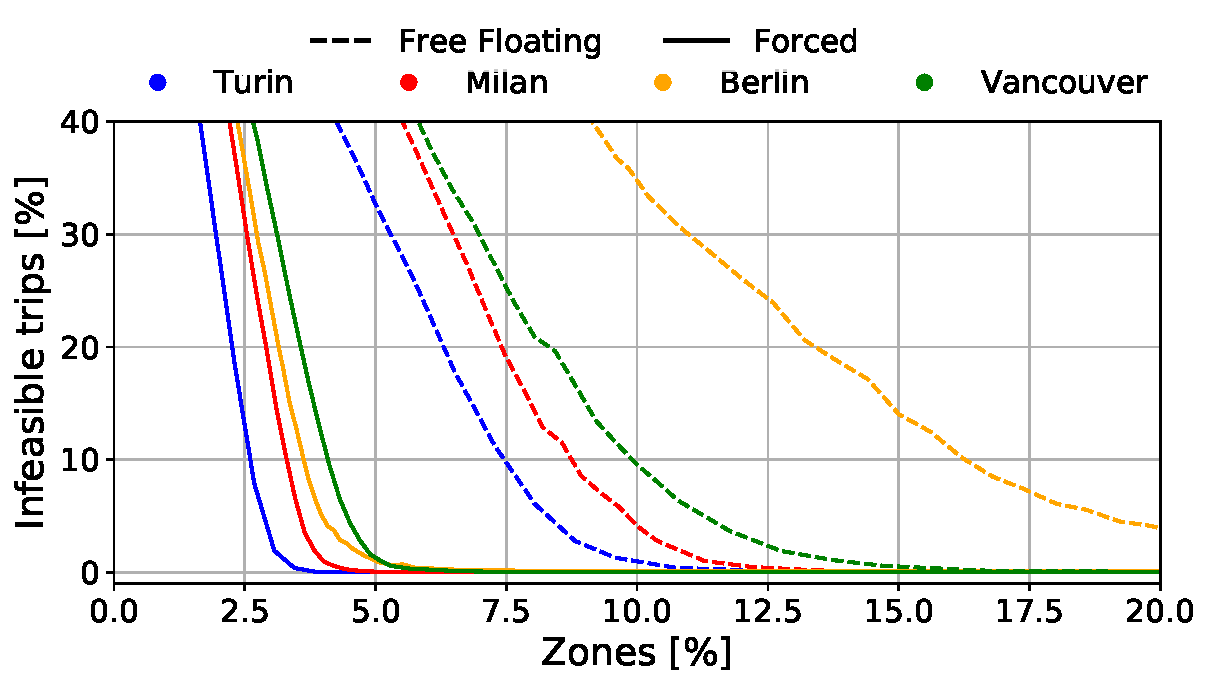
\includegraphics[width=0.95\columnwidth]{figures/DeathsVsZones_city.pdf}
         \caption{Infeasible trips when comparing the Free Floating vs Forced return policies. Forcing customer to charge when $c<\pi$ drastically improves performance.}
         \label{fig:zone_vs_deaths_FF_N}
\end{center}
\end{figure}

\section{Impact of return policy}
\label{sec:results}


\begin{figure}[t!]
  \begin{center}
	 
\includegraphics[width=0.49\textwidth]{figures/legenda.pdf}
  \vspace{-1cm}
  \end{center}
    \begin{center}
         \begin{subfigure}{0.49\textwidth}
             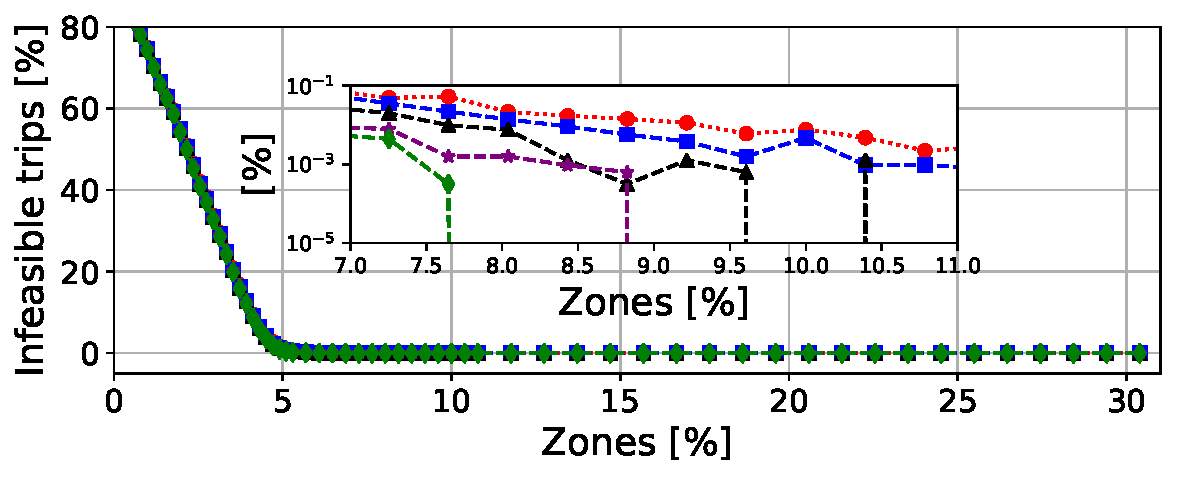
\includegraphics[width=\columnwidth]{figures/cut_Vancouver_DeathsVsZones_Policy_44_tt-25_100_4.pdf}
             \caption{Vancouver}
             \label{fig:zone_vs_deaths_vancouver_willingness}
         \end{subfigure}         
         \begin{subfigure}{0.49\textwidth}
             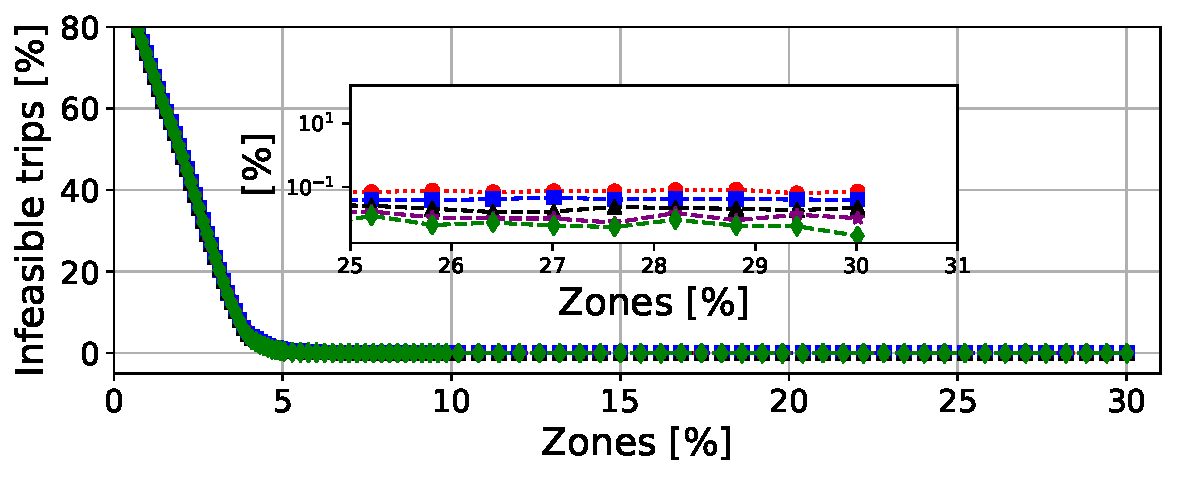
\includegraphics[width=\columnwidth]{figures/cut_Berlino_DeathsVsZones_Policy_44_tt-25_100_4.pdf}
             \caption{Berlin}
             \label{fig:zone_vs_deaths_berlino_willingness}
         \end{subfigure}
         \caption{Impact of customer willingness to cooperate $w$. Albeit the small impact, the higher $w$ is, the better it is.}
         \label{fig:zone_vs_deaths_willingness}
\end{center}
\end{figure}
I now investigate the impact of the different return policies described in section \ref{sec:5_4_return_policy}. In particular, I quantify the implications of asking customers to return the car to a different zone than the desired one when the battery is below a critical level.

\subsection{Impact on infeasible trips}

Figure~\ref{fig:cdf_characterization} has already showed that trips are typically limited. This is instrumental to choose a proper minimum charging threshold $\pi$. In particular $\pi$ must guarantee to cover the maximum trip distance and the corresponding energy being consumed. For instance, a maximum distance of 20\,km correspond to about 15\% of battery capacity for the considered car model. In the following, I take a conservative approach and set the minimum battery charge threshold $\pi=25\%$. To make results comparable, I keep the same threshold also for Berlin, where the maximum traveled distance grows to 39\,km, i.e., suggesting $\pi\geq 30\%$. Here the choice is not conservative.

As before, I focus on the infeasible trips percentage with respect to $N$. I compare the results for the Free Floating and the Forced policies. 
Figure~\ref{fig:zone_vs_deaths_FF_N} shows the results. The Forced policy (solid lines) performs much better with respect to the original Free Floating policy (dashed lines). In a nutshell, adopting a policy which mandates customers to charge the car when battery level gets below a threshold drastically reduces the number of infeasible trips, even with a handful of  charging stations. Indeed, in all cities is present a negligible percentage of infeasible trips ($< 0.1 \%$) with more than 8\% of zones equipped with charging stations.

\begin{figure*}[t!]
    \begin{center}
        \begin{subfigure}{\textwidth}
		    \begin{center}
       		    
\includegraphics[width=0.49\textwidth]{figures/legenda.pdf}
                \vspace{-0.1cm}
       	    \end{center}
            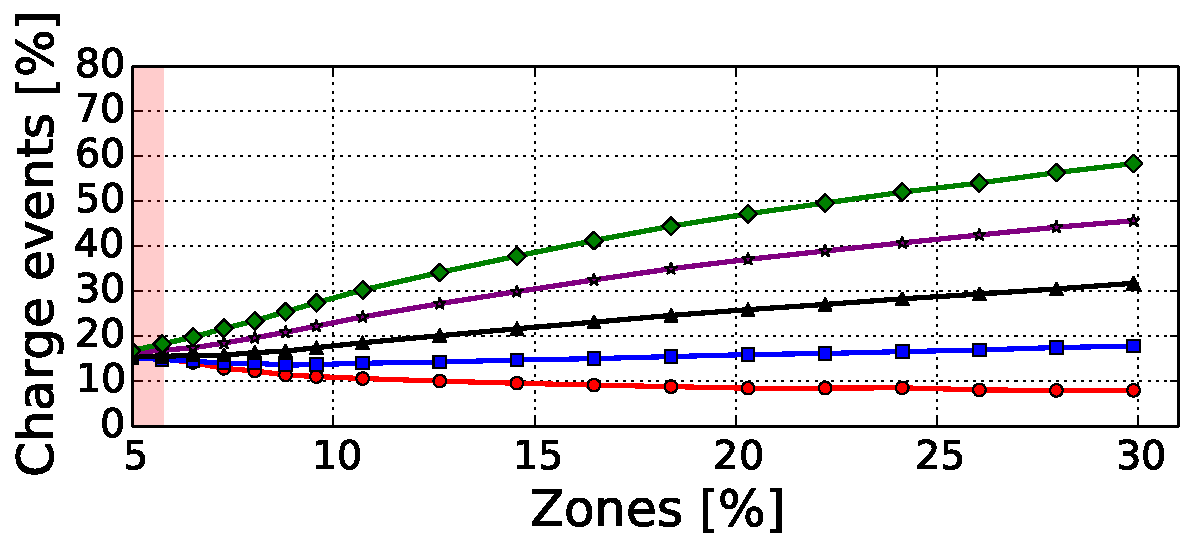
\includegraphics[width=0.33\textwidth]{figures/cut_Torino_AmountRechargePercVsZones_Policy_44_tt-25_100_4.pdf}
            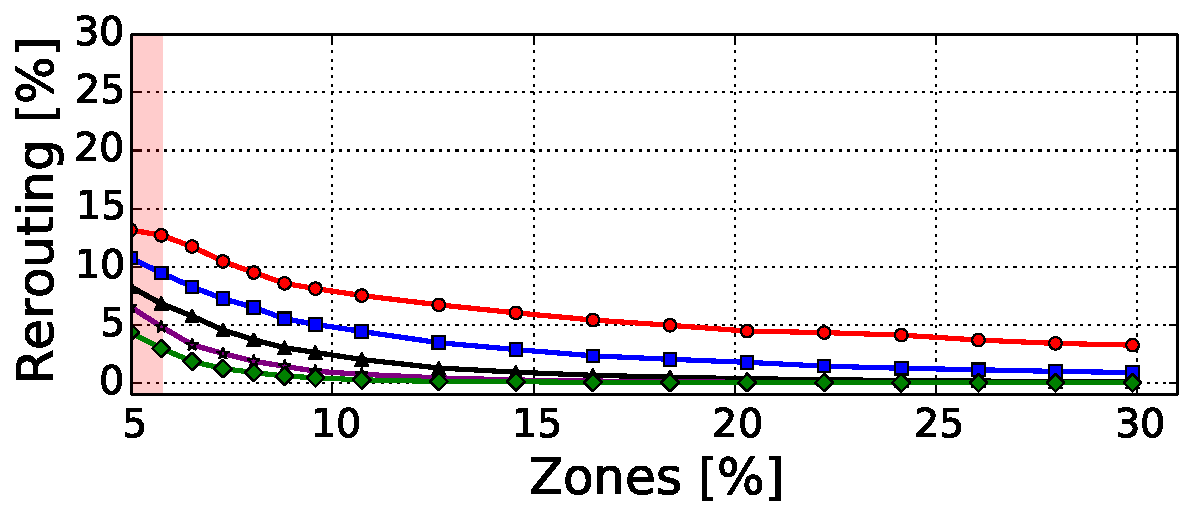
\includegraphics[width=0.33\textwidth]{figures/cut_Torino_ReroutePercVsZones_Policy_44_tt-25_100_4.pdf}
            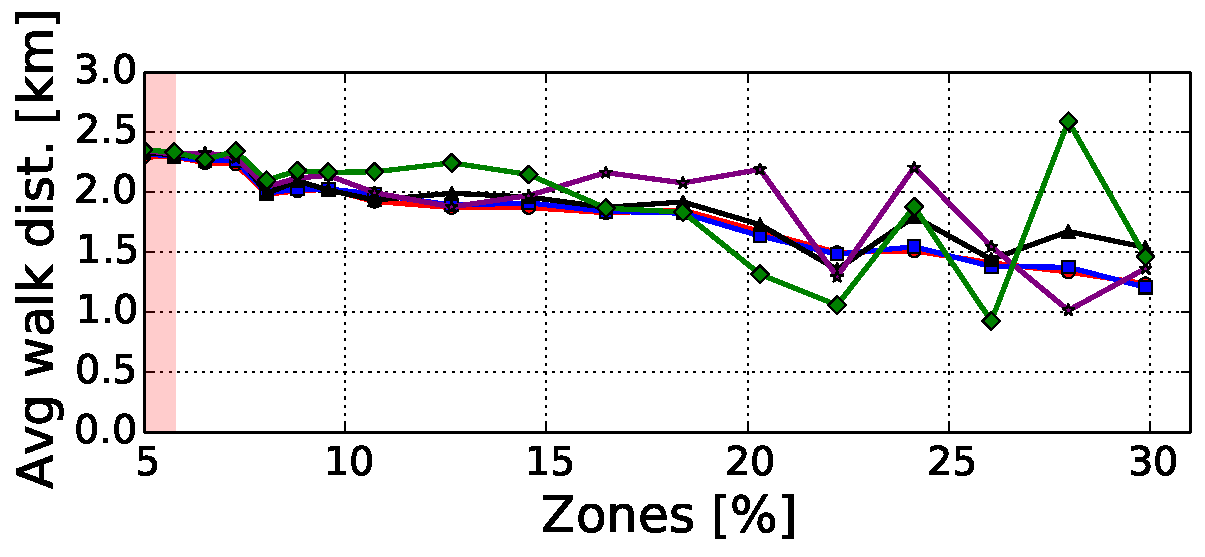
\includegraphics[width=0.33\textwidth]{figures/cut_Torino_AvgWalkedDistanceVsZones_Policy_44_tt-25_100_4.pdf}
            \caption{Turin}
            \label{fig:zone_vs_metric_torino}
        \end{subfigure}
         \begin{subfigure}{\textwidth}
            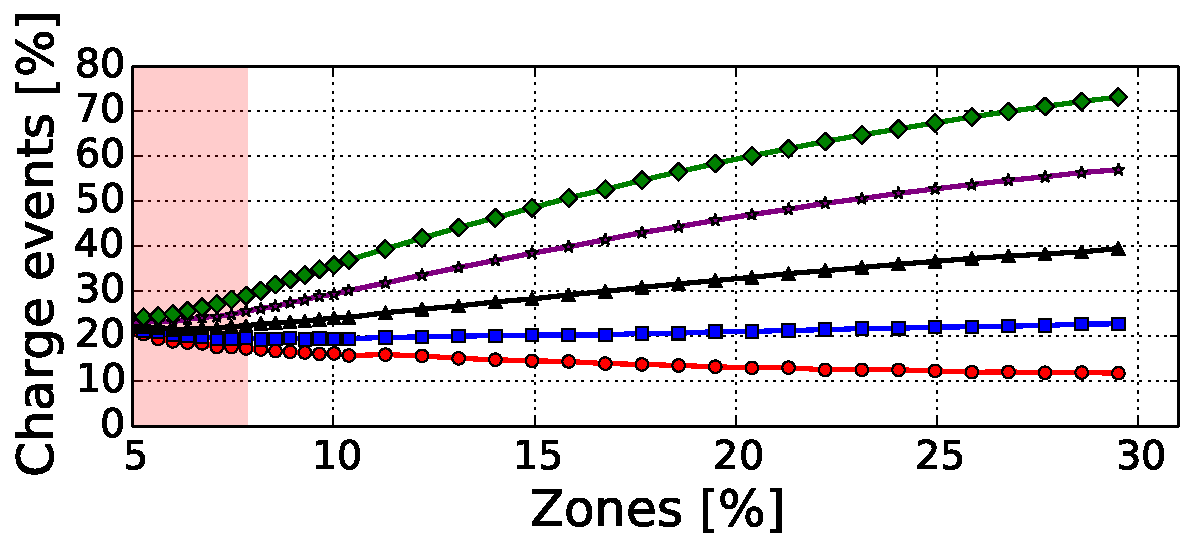
\includegraphics[width=0.33\textwidth]{figures/cut_Milano_AmountRechargePercVsZones_Policy_44_tt-25_100_4.pdf}
            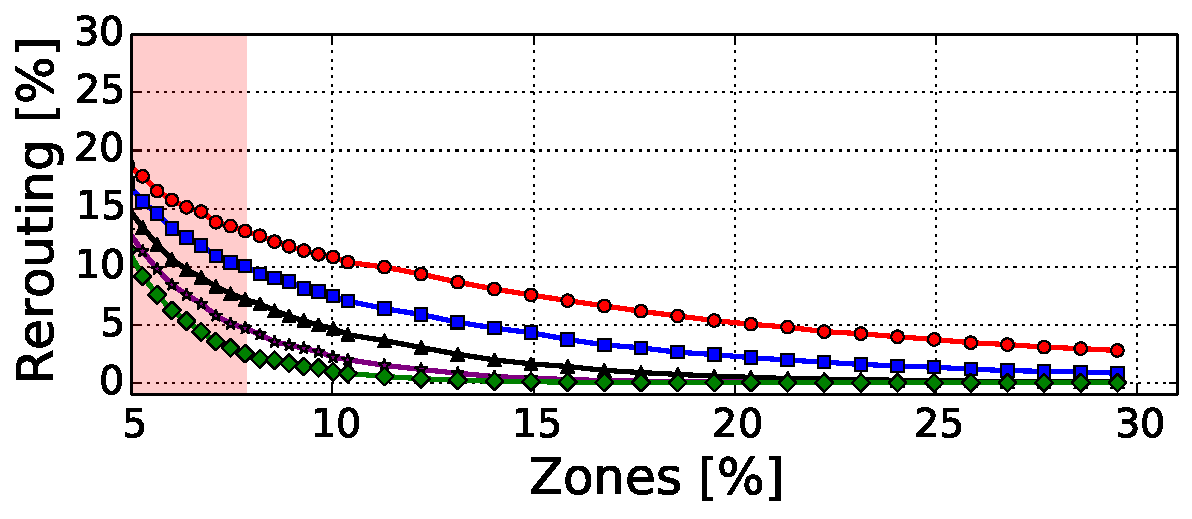
\includegraphics[width=0.33\textwidth]{figures/cut_Milano_ReroutePercVsZones_Policy_44_tt-25_100_4.pdf}
            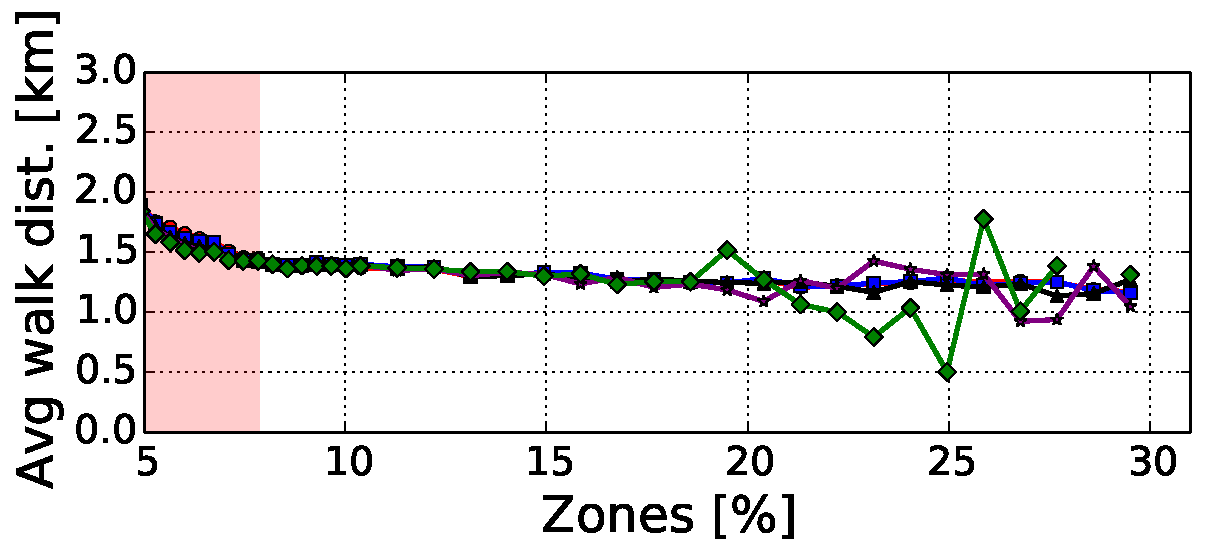
\includegraphics[width=0.33\textwidth]{figures/cut_Milano_AvgWalkedDistanceVsZones_Policy_44_tt-25_100_4.pdf}
             \caption{Milan}
             \label{fig:zone_vs_metric_milano}
         \end{subfigure}
         \begin{subfigure}{\textwidth}
         	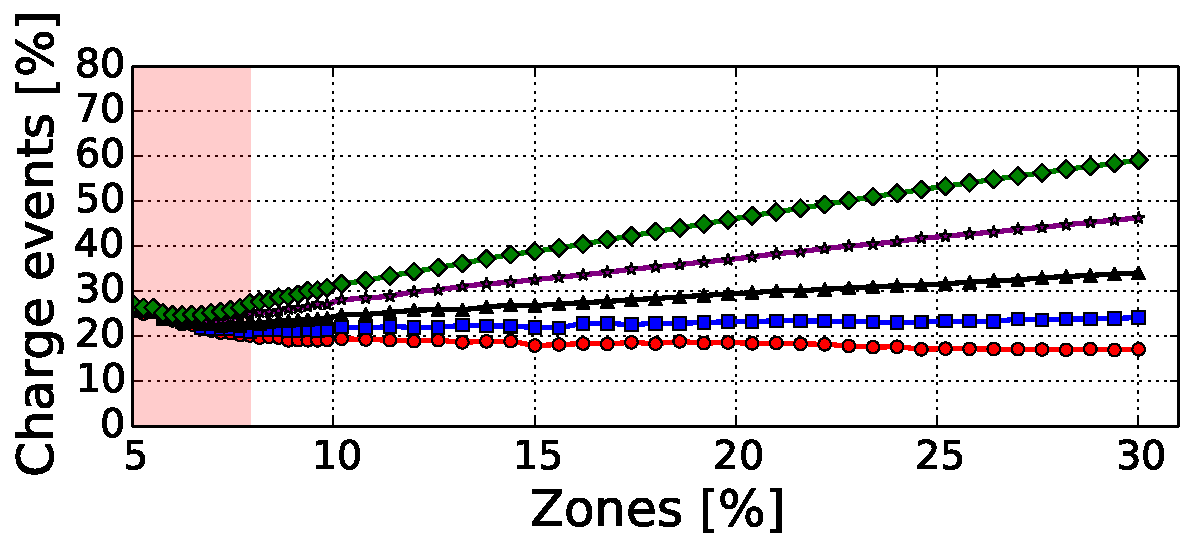
\includegraphics[width=0.33\textwidth]{figures/cut_Berlino_AmountRechargePercVsZones_Policy_44_tt-25_100_4.pdf}
            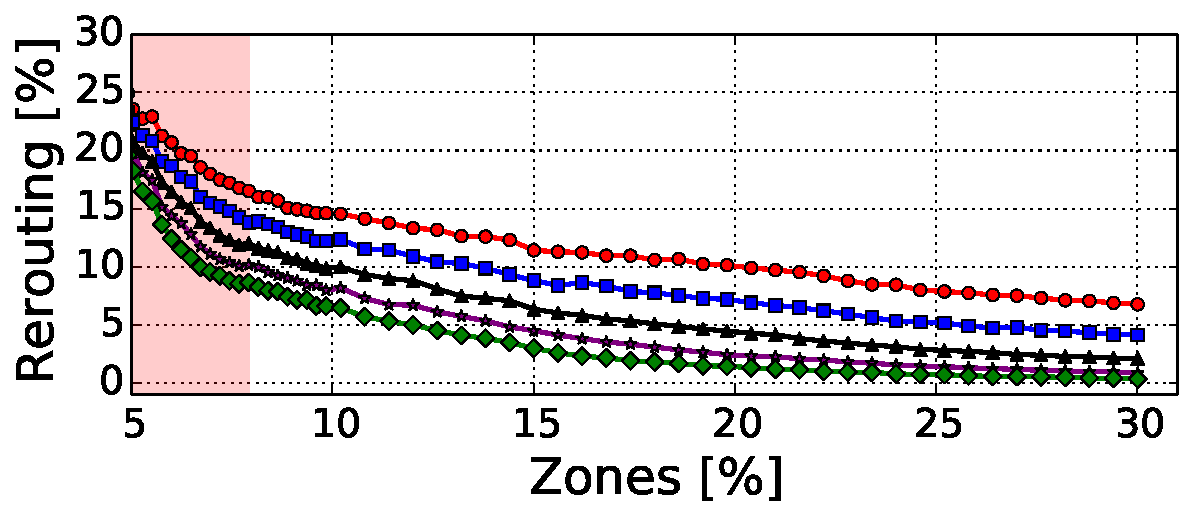
\includegraphics[width=0.33\textwidth]{figures/cut_Berlino_ReroutePercVsZones_Policy_44_tt-25_100_4.pdf}
            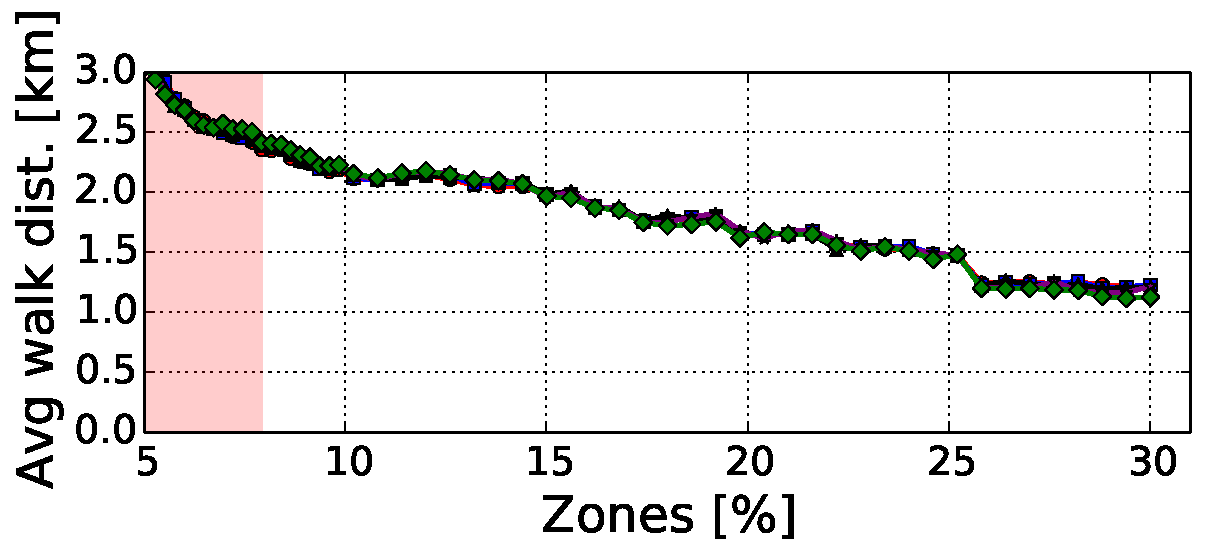
\includegraphics[width=0.33\textwidth]{figures/cut_Berlino_AvgWalkedDistanceVsZones_Policy_44_tt-25_100_4.pdf}
             \caption{Berlin}
             \label{fig:zone_vs_metric_berlino}
         \end{subfigure}
         \begin{subfigure}{\textwidth}
        	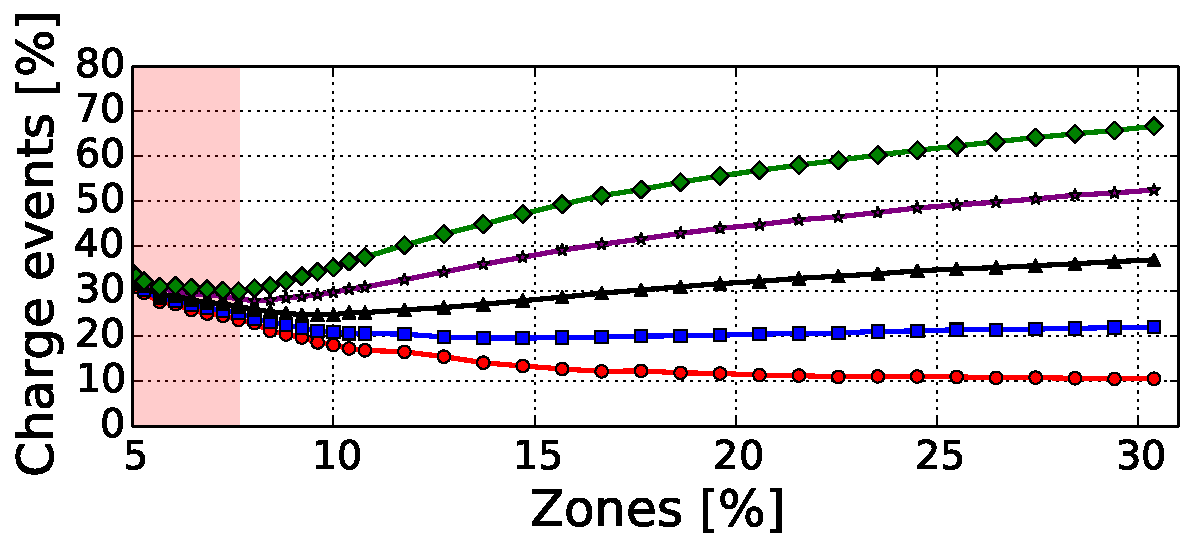
\includegraphics[width=0.33\textwidth]{figures/cut_Vancouver_AmountRechargePercVsZones_Policy_44_tt-25_100_4.pdf}
            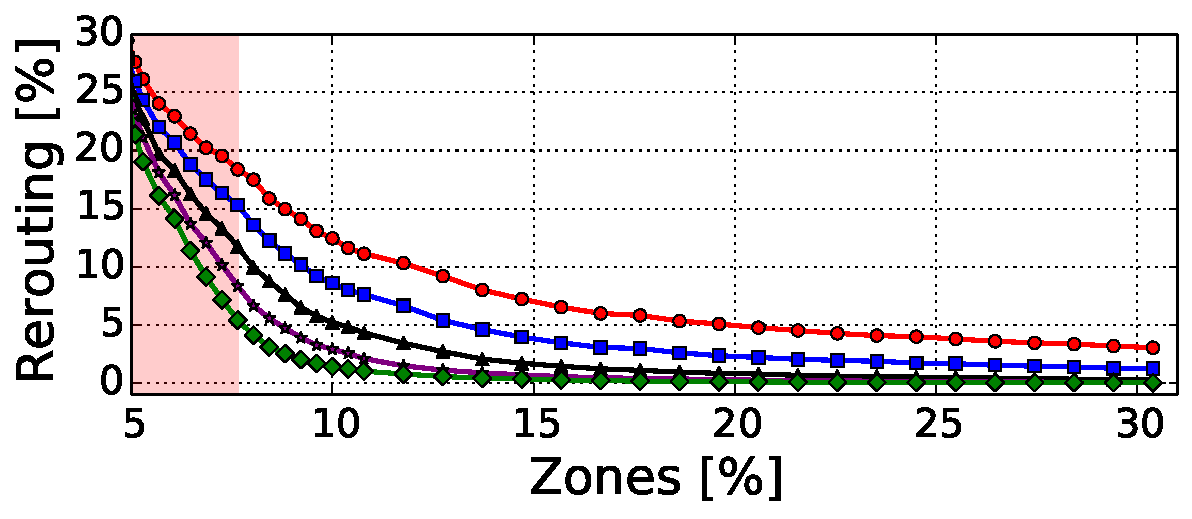
\includegraphics[width=0.33\textwidth]{figures/cut_Vancouver_ReroutePercVsZones_Policy_44_tt-25_100_4.pdf}
            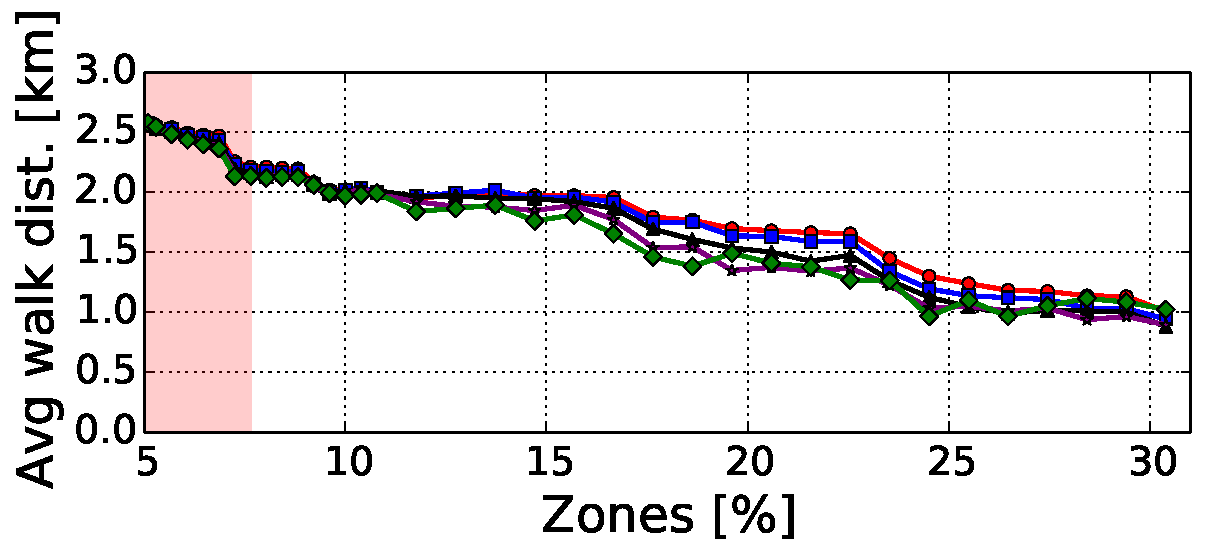
\includegraphics[width=0.33\textwidth]{figures/cut_Vancouver_AvgWalkedDistanceVsZones_Policy_44_tt-25_100_4.pdf}
             \caption{Vancouver}
             \label{fig:zone_vs_metric_vancouver}
         \end{subfigure}         
         \caption{Charge events percentage (left), re-route events percentage (middle) and walk distance averaged over re-routed trips (right),  per city. Increasing $w$ benefits the customers' experience by reducing the re-routing events significantly, but increasing the charging events.}
         \label{fig:zone_vs_metric}
\end{center}
\end{figure*}

I now focus on the impact of the willingness $w$ in the Hybrid policy. I want to understand if the more altruistic are the customers, the higher are the benefits for the system.

Figure.~\ref{fig:zone_vs_deaths_willingness} details the percentage of infeasible trips with a different willingness probability for Vancouver and Berlin. Turin and Milan are similar to Vancouver and not reported for the sake of brevity. The figures show that increasing $w$ has very little impact on the percentage of infeasible trips. Only by looking at the insets that offer a zoom in log-scale, it is possible to observe that an increasing willingness reduces infeasible trips, which are however already a marginal percentage of trips. This is due to the higher average battery level, obtained by supposing the Free Floating policy on the not of the Forced one.
In Berlin, some infeasible trips are still present even when 30\% of zones are equipped with charging stations. This is due to the maximum length of the trips, confirming the need to increase the threshold $\pi$. 
%This confirms that to eliminate the possibility of infeasible trips in Berlin, $\pi$ should be increased.

\textbf{Takeaway:} Asking customers to return the car to a charging station when the battery level goes below a minimum level drastically improves system efficiency. With just 8\% of zone covered by charging stations, the systems becomes in all the cities almost self-sustained.

\subsection{Impact on customer experience}

As there is no strong evidence that the overall system would perform better with customers' altruistic behaviour, here I check benefits on the customer experience. Forcing a customer to park in a charging station can be annoying, because the customer has to reach the charging station, and lose time to plug and unplug the car to and from the pole. Even worse, re-routing customers to other zones for charging increases the distances they have to walk to reach their desired destination.
In the following, I measure the customer's experience through the KPIs described in \ref{sec:5_5_kpi_scenario}.

Figure.~\ref{fig:zone_vs_metric} reports, for each city, and for different willingness the percentage of charge events (left plots), the percentage of re-route events (middle plots), and the average walk distance when re-routed (right plots). In all graphs the shaded area highlights the infeasible region, i.e., when infeasible trips are higher than 0.1\% in at least a case. The lack of charging zones creates artifacts here. 

Focus first on the charge percentage - leftmost plots. When the number of charging stations is close to the minimum, most poles are occupied by cars that have been forced to charge. This leaves little room for opportunistic charges, and there is little impact of $w$. For increasing number of charging stations, the opportunity to find a free pole in $o(i)$ increases. Thus, the higher is $w$, the higher are the recharging events. Correspondingly, the average battery charge increases -- see Fig.~\ref{fig:zone_vs_soc_vancouver}.

Interestingly, the charge percentage decreases for a selfish customer ($w=0$), reaching about 5-8\% for sufficiently large number of charging stations. This corresponds to the average number of charges per car that guarantees minimum battery charge of 25\%. Indeed, given the average rental distance of 5\,km (Table~\ref{tab:summary}) and battery range of 100.5\,km (at the net of the safety threshold $\pi$), a car could sustain on average 20 normal trips before needing to charge.  

Move now to the percentage of re-routing events - middle plots in figure.~\ref{fig:zone_vs_metric}. Two important effects are visible. First, re-routing probability decreases as expected: the more the stations are, the more likely customers find a charging station at their desired final zone. With selfish behaviour ($w=0$), the fraction of re-routing events remains large even for large $N$.
Second, the more collaborative are customers, the better it is for the entire system. With half of customers that return voluntarily the car to charging station if present in their final destination, for Milan, Turin and Vancouver the re-routings are less than 1\% with 18\% of charging zones. These can be handled by a relocation policy, i.e., the system could take care to charge those less than 1\% of cars whose battery level is close to $\pi$. Note that this corresponds to maximum 53 relocation events per day. Instead, for Berlin the number of re-routing remains larger than 3\%, mainly due to its larger size.



At last focus on the average walk distance when the car is re-routed -- rightmost plots in figure.~\ref{fig:zone_vs_metric}. When forced to charge to a different zone than the desired one, customers would be asked to drive far, a likely unacceptable penalty unless mitigated by offering incentives to customers, e.g., offering a free rental when re-routed.\footnote{The noise for large $N$ is due to the very small number of re-routing events.} Notice that by increasing the number of charging stations, the walked distance is reduced, but not linearly. This is also due to the fact that charging stations are not placed uniformly in space, following the number of parking heuristic. 



Therefore, I would like to have $w=1$ to reduce (far) re-routings and infeasible trips, and $w=0$ to reduce charging events. In an attempt to take into consideration both aspects, I compute the (global) walk distance averaged over all trips. This considers the penalty due to (i) the re-routing events, and (ii) the walk distance when charging in a pole of the desired final destination (pole distance would be 150\,m, on average).
Figure.~\ref{fig:zone_vs_wwd_vancouver} reports this general average walk distance for Vancouver. For more than 10\% of zones with charging stations, with all the policies customers have to walk on average less than 400\,m.
%. This considers the penalty due to (i) the rerouting events, and (ii) for opportunistically charging to a pole in the final zone.
%For the second case, we need to compute the average in-zone distance from the recharging stations (placed at the center) and all possible destinations within the same zone. Assuming a square of $500\,m$ side, the average distance from the center is about $150\,m$.
When the number of charging station is low, increasing $w$ reduces the average walking distance, since opportunistic charges reduce re-routing events. However, increasing the number of charging zones increases the cost of always driving to a pole in the same zone. In the case of Vancouver, after 23\% of zones, the best policy switches from $w=1$ to $w=0$. Therefore, the policy to use may be different according to the number of charging stations. Overall, for all the four cities and 10\% of zones, and choosing the policy with $w=1$, customers in average walk less than 200\,m to reach their desired destination.

\textbf{Takeaway:} Hybrid policy significantly reduces the number of times the customer has to drive to a charging station in a different zone than the desired one. However, it increases the number of times the customer parks at a charging station and has to plug the car to the pole. Therefore, one must  be cautious when weighting these results and designing the return policies which impact the customers. 


\begin{figure}[t!]
    \begin{center}
	    
\includegraphics[width=0.47\textwidth]{figures/legenda.pdf}
    \vspace{-0.1cm}
    \end{center}
    \begin{center}
        \begin{subfigure}{0.47\textwidth}
            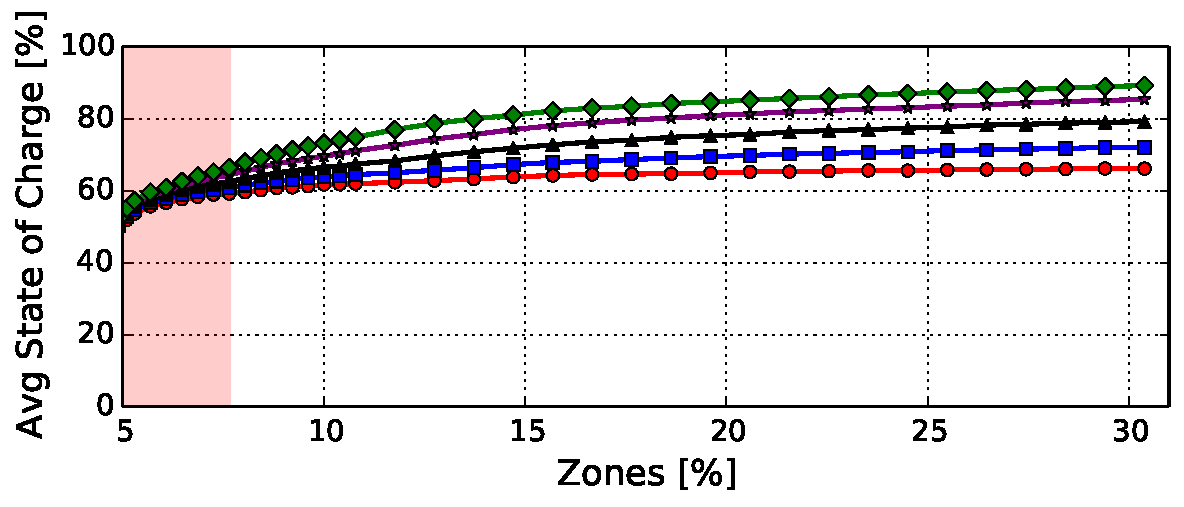
\includegraphics[width=\columnwidth]{figures/cut_Vancouver_AvgSOCVsZones_Policy_44_tt-25_100_4.pdf}
            \caption{Average State of Charge - the higher the better.}
            \label{fig:zone_vs_soc_vancouver}
        \end{subfigure}
         \begin{subfigure}{0.47\textwidth}
            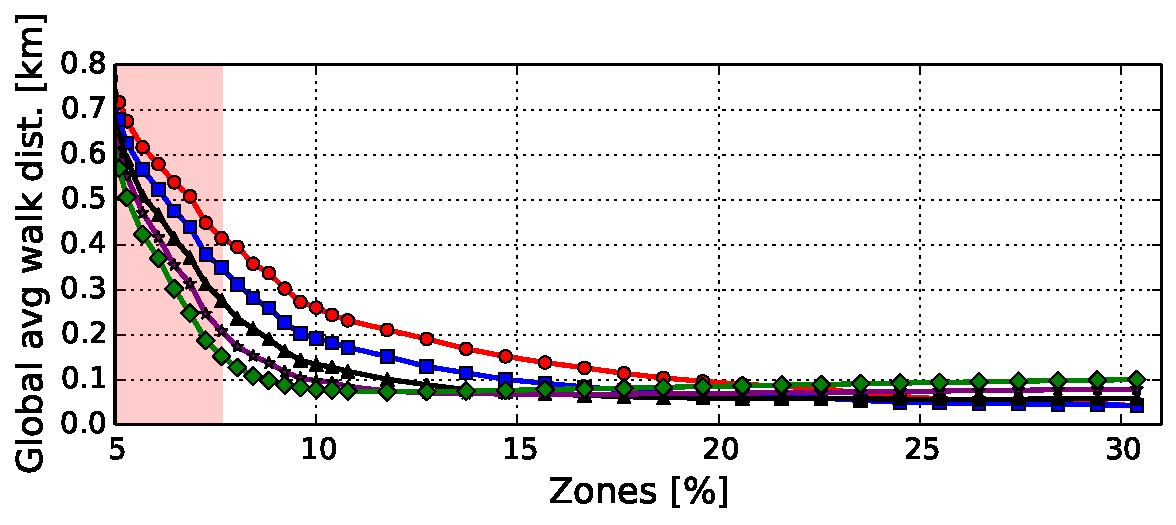
\includegraphics[width=\columnwidth]{figures/cut_Vancouver_TravelWithPenlatyVsZones_Policy_44_tt-25_100_4.pdf}
             \caption{Global average walk distance - the lower the better.}
             \label{fig:zone_vs_wwd_vancouver}
         \end{subfigure}
         \caption{Details of the average battery charge status and global average walk distance for Vancouver. Other cities have similar results.}
         \label{fig:discomoft_metrics_vancouver}
\end{center}
\end{figure}



